\documentclass[8pt,a4paper,compress]{beamer}

\usepackage{/home/siyer/lib/slides}

\title{Data Abstraction}
\date{}

\begin{document}
\begin{frame}
\vfill
\titlepage
\end{frame}

\begin{frame}
\frametitle{Outline}
\tableofcontents
\end{frame}

\section{Using Abstract Data Types}
\begin{frame}[fragile]
\pause

An abstract data type (ADT) is one whose representation is hidden from the client

\pause
\bigskip

We use an API to specify the behavior of an ADT

\pause
\bigskip

Example (a comparable \lstinline{Counter} data type)
\begin{center}
\begin{tabular}{cc}
method & description \\ \hline
\lstinline$Counter(String id)$ & create a counter named $id$ \\
\lstinline$void increment()$ & increment the counter by one \\
\lstinline$int tally()$ & number of increments since creation \\
\lstinline$String toString()$ & string representation of the counter \\
\lstinline$int compareTo(Counter that)$ & compare the counter to $that$
\end{tabular} 
\end{center}
\end{frame}

\begin{frame}[fragile]
\pause

Similarities with a library of static methods
\begin{itemize}
\item Both are implemented as a Java class
\item Instance methods may take zero or more arguments of a specified type, separated by commas and enclosed in parentheses
\item They may provide a return value of a specified type or no return value (signified by \lstinline{void})
\end{itemize}

\pause
\bigskip

Differences from a library of static methods
\begin{itemize}
\item Some entries (called constructors) have the same name as the class and lack a return type
\item Instance methods lack the \lstinline{static} modifier, and their purpose is to operate on data type values
\item Some instance methods are inherited from parent classes
\end{itemize}
\end{frame}

\begin{frame}[fragile]
\pause

Every Java data type inherits from \lstinline{java.lang.Object}, the \lstinline{toString()}, \lstinline{equals()}, and \lstinline{hashCode()} methods

\pause
\bigskip

An object is an entity that can take on a data-type value

\pause
\bigskip

An object is characterized by its state (values from its data type), identity (place in memory), and behavior (effect of data-type operations)

\pause
\bigskip

To create (or instantiate) an object, we invoke a constructor using the keyword \lstinline{new} followed by the class name, followed by 0 or more arguments, enclosed in parentheses and separated by commas

\begin{lstlisting}[language=Java]
Counter heads = new Counter("heads");
Counter tails = new Counter("tails");
\end{lstlisting}

\pause
\bigskip

Object representation in memory
\begin{center}
\visible<6->{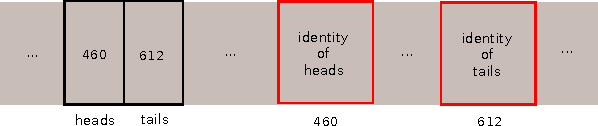
\includegraphics[scale=0.8]{./figures/obj_rep.pdf}}
\end{center}
\end{frame}

\begin{frame}[fragile]
\pause

The purpose of an instance method is to operate on data-type values

\pause
\bigskip

An instance method is invoked as object name, followed by a period, followed by the method name, followed by 0 or more arguments, enclosed in parentheses and separated by commas

\pause
\bigskip

Example (simulating $T$ coin flips)

\begin{lstlisting}[language=Java]
import edu.princeton.cs.algs4.Counter;
import edu.princeton.cs.algs4.StdOut;
import edu.princeton.cs.algs4.StdRandom;

public class Flips {
    public static void main(String[] args) {
        int T = Integer.parseInt(args[0]);
        Counter heads = new Counter("heads");
        Counter tails = new Counter("tails");
        for (int t = 0; t < T; t++) {
            if (StdRandom.bernoulli(0.5)) { heads.increment(); }
            else { tails.increment(); }
        }
        StdOut.println(heads);
        StdOut.println(tails);
        int delta = heads.tally() - tails.tally();
        StdOut.println("delta: " + Math.abs(delta));
    }
}
\end{lstlisting}

\pause

\begin{lstlisting}[language={}]
$ java Flips 1000000
499422 heads
500578 tails
delta: 1156
\end{lstlisting}
\end{frame}

\begin{frame}[fragile]
\pause

An assignment statement with a reference type creates a copy (an alias) of the reference, not a new object

\pause
\bigskip

We can pass objects as arguments to methods and can also use an object as a return value from a method

\pause
\bigskip

Example (simulating $T$ coin flips and finding out if heads or tails is the winner)
\begin{lstlisting}[language=Java]
import edu.princeton.cs.algs4.Counter;
import edu.princeton.cs.algs4.StdOut;
import edu.princeton.cs.algs4.StdRandom;

public class FlipsMax {
    public static Counter max(Counter x, Counter y) {
        return x.tally() > y.tally() ? x : y;
    }

    public static void main(String[] args) {
        int T = Integer.parseInt(args[0]);
        Counter heads = new Counter("heads");
        Counter tails = new Counter("tails");
        for (int t = 0; t < T; t++) {
            if (StdRandom.bernoulli(0.5)) { heads.increment(); }
            else { tails.increment(); }
        }
        if (heads.tally() == tails.tally()) { StdOut.println("Tie"); }
        else { StdOut.println(max(heads, tails) + " wins"); }
    }
}
\end{lstlisting}

\pause

\begin{lstlisting}[language={}]
$ java FlipsMax 1000000
501181 heads wins
\end{lstlisting}
\end{frame}

\begin{frame}[fragile]
\pause

In Java, every value of any nonprimitive type is an object, and in particular, arrays are objects 

\pause
\bigskip

Array entries can be of any type, including reference types, ie, they can be objects

\pause
\bigskip

Example (simulating $T$ rolls of a die)

\begin{lstlisting}[language=Java]
import edu.princeton.cs.algs4.Counter;
import edu.princeton.cs.algs4.StdOut;
import edu.princeton.cs.algs4.StdRandom;

public class Rolls {
    public static void main(String[] args) {
        int T = Integer.parseInt(args[0]);
        int SIDES = 6;
        Counter[] rolls = new Counter[SIDES + 1];
        for (int i = 1; i <= SIDES; i++) { rolls[i] = new Counter(i + "'s"); }
        for (int t = 0; t < T; t++) {
            int result = StdRandom.uniform(1, SIDES + 1);
            rolls[result].increment();
        }
        for (int i = 1; i <= SIDES; i++) { StdOut.println(rolls[i]); }
    }
}
\end{lstlisting}

\pause

\begin{lstlisting}[language={}]
$ java Rolls 1000000
166674 1's
166337 2's
166566 3's
166926 4's
166822 5's
166675 6's
\end{lstlisting}
\end{frame}

\section{Examples of Abstract Data Types}
\begin{frame}[fragile]
\pause

Standard Java system types in \lstinline{java.lang}
\begin{center}
\begin{tabular}{cc}
type & description \\ \hline
\lstinline$Integer$ & \lstinline$int$ wrapper \\
\lstinline$Double$ & \lstinline$double$ wrapper \\
\lstinline$String$ & indexed chars \\
$\dots$ & $\dots$
\end{tabular} 
\end{center}

\pause

Other Java Types
\begin{center}
\begin{tabular}{cc}
type & description \\ \hline
\lstinline$java.awt.Color$ & colors \\
\lstinline$java.net.URL$ & URLs \\
\lstinline$java.io.File$ & files \\
$\dots$ & $\dots$
\end{tabular} 
\end{center}

\pause

File IO types from \lstinline{edu.princeton.cs.algs4}
\begin{center}
\begin{tabular}{cc}
type & description \\ \hline
\lstinline$In$  & input stream \\
\lstinline$Out$ & output stream \\
$\dots$ & $\dots$
\end{tabular} 
\end{center}

\pause

Data-oriented types from \lstinline{edu.princeton.cs.algs4}
\begin{center}
\begin{tabular}{cc}
type & description \\ \hline
\lstinline$Date$ & date \\
\lstinline$Transaction$ & transaction \\
$\dots$ & $\dots$
\end{tabular} 
\end{center}
\end{frame}

\begin{frame}[fragile]
\pause

Types for analysis of algorithms from \lstinline{edu.princeton.cs.algs4}
\begin{center}
\begin{tabular}{cc}
type & description \\ \hline
\lstinline$Counter$ &  counter \\
\lstinline$Stopwatch$ & stopwatch \\
$\dots$ & $\dots$
\end{tabular} 
\end{center}

\pause

Collection types from \lstinline{edu.princeton.cs.algs4}
\begin{center}
\begin{tabular}{cc}
type & description \\ \hline
\lstinline$LinkedBag$ & bag \\
\lstinline$LinkedStack$ & pushdown stack \\
$\dots$ & $\dots$
\end{tabular} 
\end{center}

\pause

Data-oriented graph types from \lstinline{edu.princeton.cs.algs4}
\begin{center}
\begin{tabular}{cc}
type & description \\ \hline
\lstinline$Graph$  & undirected graph \\
\lstinline$Digraph$ & directed graph \\
$\dots$ & $\dots$
\end{tabular} 
\end{center}

\pause

Operations-oriented graph types from \lstinline{edu.princeton.cs.algs4}
\begin{center}
\begin{tabular}{cc}
type & description \\ \hline
\lstinline$UF$ & dynamic connectivity \\
\lstinline$DepthFirstPaths$ & depth-first path searcher \\
$\dots$ & $\dots$
\end{tabular} 
\end{center}
\end{frame}

\begin{frame}[fragile]
\pause
The \lstinline{String} data type represents an indexed sequence of \lstinline{char} values

\begin{center}
\begin{tabular}{cc}
method & description \\ \hline
\lstinline$String()$ & create an empty string \\
\lstinline$int length()$ & length of the string \\
\lstinline$char charAt(int i)$ & $i$th character \\
\lstinline$int indexOf(String p)$ & first occurrence of $p$ or -1 \\ \lstinline$int indexOf(String p, int i)$ & first occurrence of $p$ after $i$ or -1 \\
\lstinline$String concat(String t)$ & the string with $t$ appended \\
\lstinline$String substring(int i, int j)$ & substring of the string from $i$ (inclusive) to $j$ (exclusive) \\
\lstinline$String[] split(String delim)$ & strings between occurrences of $delim$ \\
\lstinline$int compareTo(String t)$ & compare the string to $t$ \\
\lstinline$boolean equals(String t)$ & is the string's value the same as $t$'s? \\
$\dots$ & $\dots$
\end{tabular} 
\end{center}

\pause
\bigskip

Example (testing if a string is a palindrome)
\begin{lstlisting}[language=Java]
public static boolean isPalindrome(String s) {
    if (s.length() == 0) {
        return true;
    } 
    return s.charAt(0) == s.charAt(s.length() - 1) && 
        isPalindrome(s.substring(1, s.length() - 1));
}
\end{lstlisting}
\end{frame}

\begin{frame}[fragile]
\begin{minipage}{250pt}
\pause

Consider an input sequence of pairs of integers, where each integer represents an object of some type, and the pair $(p, q)$ means that ``$p$ is connected to $q$''

\pause
\bigskip

The goal of the dynamic connectivity problem is to devise a data structure to decide whether or not a new pair of objects is connected 

\pause
\bigskip

The \lstinline{UF} union-find data type provides that data structure

\begin{center}
\begin{tabular}{cc}
method & description \\ \hline
\lstinline$UF(int N)$ & \makecell{initialize an empty union-find data \\ structure with $N$ sites} \\
\lstinline$int find(int p)$ & \makecell{component identifier \\ for $p$ (0 to $N-1$)} \\
\lstinline$int count()$ & number of components \\
\lstinline$boolean connected(int p, int q)$ & are $p$ and $q$ in the same component? \\
\lstinline$void union(int p, int q)$ & add connection between $p$ and $q$
\end{tabular} 
\end{center} 
\end{minipage}%
\begin{minipage}{60pt}
\hfill \visible<2->{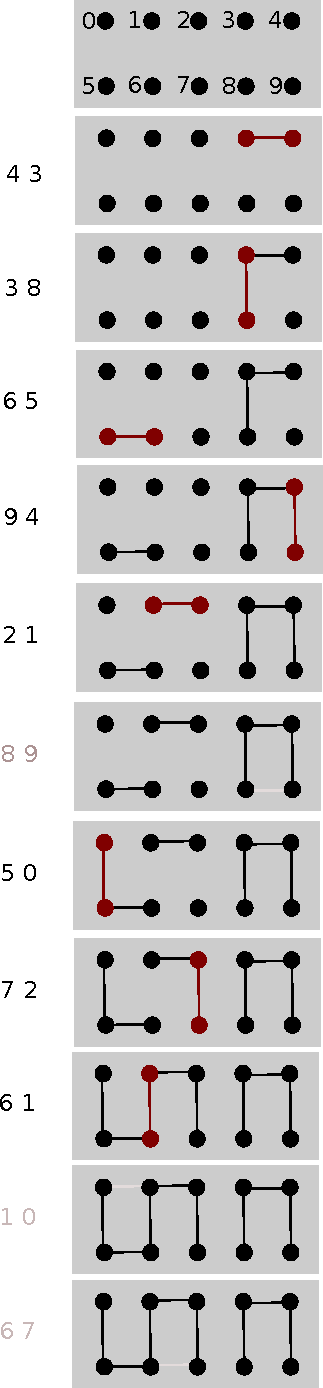
\includegraphics[scale=0.35]{./figures/dyn_conn.pdf}}
\end{minipage}
\end{frame}

\begin{frame}[fragile]
\begin{minipage}{250pt}

\pause
\smallskip

\lstinline{UF} client
\begin{lstlisting}[language=Java]
import edu.princeton.cs.algs4.WeightedQuickUnionUF;
import edu.princeton.cs.algs4.StdIn;
import edu.princeton.cs.algs4.StdOut;

public class UFClient {
    public static void main(String[] args) {
        int N = StdIn.readInt();
        WeightedQuickUnionUF uf = new WeightedQuickUnionUF(N);
        while (!StdIn.isEmpty()) {
            int p = StdIn.readInt();
            int q = StdIn.readInt();
            if (uf.connected(p, q)) { continue; }
            uf.union(p, q);
            StdOut.println(p + " " + q);
        }
        StdOut.println(uf.count() + " components");
    }
}
\end{lstlisting}
    
\pause

\begin{lstlisting}[language={}]
$ more tinyUF.txt
10 4 3 3 8 6 5 9 4 2 1 8 9 5 0 7 2 6 1 1 0 6 7
\end{lstlisting}    

\pause

\begin{lstlisting}[language={}]
$ java UFClient < tinyUF.txt 
4 3
3 8
6 5
9 4
2 1
5 0
7 2
6 1
2 components
\end{lstlisting}
\end{minipage}%
\begin{minipage}{60pt}
\hfill \visible<2->{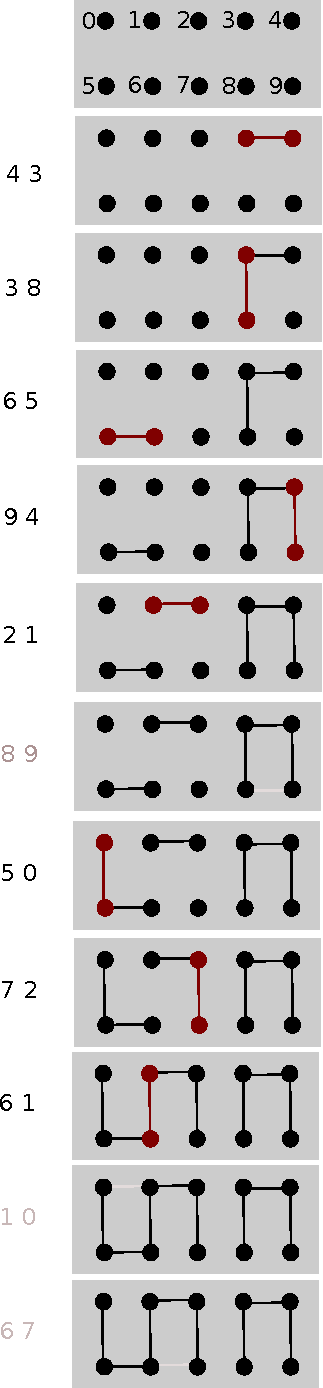
\includegraphics[scale=0.35]{./figures/dyn_conn.pdf}}
\end{minipage}
\end{frame}

\section{Implementing an Abstract Data Type}
\begin{frame}[fragile]
\pause

We implement ADTs with a Java class, putting the code (instance variable declarations, constructors, and instance methods) in a file with the same name as the class, followed by the \lstinline{.java} extension

\pause
\bigskip

Instance variables define the state of each object, and unlike local variables, each instance variable can have numerous values (one per object)

\pause
\bigskip

Constructors have the same name as the class, have no return value, and generally, their purpose is to initialize the instance variables

\pause
\bigskip

Instance methods define the behavior of each object

\pause
\bigskip

Each instance method has a return type (or \lstinline{void}), a signature, and a body

\pause
\bigskip

When a client invokes an instance method, the action is the same as for static methods, with one critical distinction: they can access and perform operations on instance variables

\pause
\bigskip

Within an instance method or a constructor, \lstinline{this} is a reference to the current object --- the object whose method or constructor is being called

\pause
\bigskip

The most common reason for using the \lstinline{this} keyword is because a field (instance variable) is shadowed by a method or constructor parameter
\end{frame}

\begin{frame}[fragile]
\pause

\lstinline{edu.princeton.cs.algs4.Counter} API
\begin{center}
\begin{tabular}{cc}
method & description \\ \hline
\lstinline$Counter(String id)$ & create a counter named $id$ \\
\lstinline$void increment()$ & increment the counter by one \\
\lstinline$int tally()$ & number of increments since creation \\
\lstinline$String toString()$ & string representation of the counter \\
\lstinline$int compareTo(Counter that)$ & compare the counter to $that$
\end{tabular} 
\end{center}

\pause

\lstinline{edu.princeton.cs.algs4.Counter} implementation
\begin{lstlisting}[language=Java]
package edu.princeton.cs.algs4;

public class Counter implements Comparable<Counter> {
    private final String id;
    private int count;

    public Counter(String id) { this.id = id; }

    public void increment() { count++; }

    public int tally() { return count; }

    public String toString() { return tally() + " " + id; }
    
    public int compareTo(Counter that) {
        if      (this.count < that.count) { return -1; }
        else if (this.count > that.count) { return +1; }
        else                              { return  0; }
    }
}
\end{lstlisting}
\end{frame}

\section{Data-type Design}
\begin{frame}[fragile]
\pause

Interface inheritance (aka subtyping) allows programmers to support different implementations for the same API, specified as an interface

\pause
\bigskip

Example (\lstinline{Factorial} interface and two different implementations for it)
\begin{center}
\begin{tabular}{cc}
method & description \\ \hline
\lstinline$int compute(int N)$ & $N!$
\end{tabular} 
\end{center}

\begin{lstlisting}[language=Java]
public class FactorialIter implements Factorial {
    public int compute(int N) {
        int result = 1;
        for (int i = 1; i <= N; i++) {
            result *= i;
        }
        return result;
    }
}
\end{lstlisting}

\begin{lstlisting}[language=Java]
public class FactorialRec implements Factorial {
    public int compute(int N) {
        return (N == 1) ? 1 : N * compute(N - 1);
    }
}
\end{lstlisting}
\end{frame}

\begin{frame}[fragile]
\pause

Comparison interfaces for defining comparable data types
\begin{itemize}
\item \lstinline{java.lang.Comparable}
\begin{center}
\begin{tabular}{cc}
method & description \\ \hline
\lstinline$int compareTo(T o)$ & \makecell{compare $this$ with $o$ for order, and return a negative \\ integer, zero, or positive integer based on the comparison}
\end{tabular} 
\end{center}

\item \lstinline{java.util.Comparator}
\begin{center}
\begin{tabular}{cc}
method & description \\ \hline
\lstinline$int compare(T o1, T o2)$ & \makecell{compare $o_1$ and $o_2$ for order, and return a negative \\ integer, zero, or positive integer based on \\ the comparison}
\end{tabular} 
\end{center}
\end{itemize}
\end{frame}

\begin{frame}[fragile]
\pause

Example (a comparable \lstinline{Planet} data type)
\begin{lstlisting}[language=Java]
import edu.princeton.cs.algs4.StdOut;
import java.util.Arrays;
import java.util.Comparator;

public class Planet implements Comparable<Planet> {
    private String name;
    private int moons;

    public Planet(String name, int moons) {
        this.name = name;
        this.moons = moons;
    }
    
    public String name() { return name; }

    public int moons() { return moons; }

    public int compareTo(Planet o) { return name.compareTo(o.name); }
    
    public String toString() { return name + ", " + moons; }

    public static class MoonOrder implements Comparator<Planet> {
        public int compare(Planet p1, Planet p2) {
            return p1.moons() - p2.moons();
        }
    }
\end{lstlisting}
\end{frame}

\begin{frame}[fragile]
\pause

\begin{lstlisting}[language=Java]
    public static void main(String[] args) {
        Planet[] planets = new Planet[8];
        planets[0] = new Planet("Mercury", 0);
        planets[1] = new Planet("Venus", 0);
        planets[2] = new Planet("Earth", 1);
        planets[3] = new Planet("Mars", 2);
        planets[4] = new Planet("Jupiter", 67);
        planets[5] = new Planet("Saturn", 62);
        planets[6] = new Planet("Uranus", 27);
        planets[7] = new Planet("Neptune", 14);
        StdOut.println("Unsorted:");
        for (int i = 0; i < planets.length; i++) {
            StdOut.println("  " + planets[i]);
        }
        Arrays.sort(planets);
        StdOut.println("Sorted by name:");
        for (int i = 0; i < planets.length; i++) {
            StdOut.println("  " + planets[i]);
        }
        Arrays.sort(planets, new Planet.MoonOrder());
        StdOut.println("Sorted by # of moons:");
        for (int i = 0; i < planets.length; i++) {
            StdOut.println("  " + planets[i]);
        }
    }
}
\end{lstlisting}
\end{frame}

\begin{frame}[fragile]
\pause

\begin{lstlisting}[language={}]
$ java Planet
Unsorted:
  Mercury, 0
  Venus, 0
  Earth, 1
  Mars, 2
  Jupiter, 67
  Saturn, 62
  Uranus, 27
  Neptune, 14
Sorted by name:
  Earth, 1
  Jupiter, 67
  Mars, 2
  Mercury, 0
  Neptune, 14
  Saturn, 62
  Uranus, 27
  Venus, 0
Sorted by # of moons:
  Mercury, 0
  Venus, 0
  Earth, 1
  Mars, 2
  Neptune, 14
  Uranus, 27
  Saturn, 62
  Jupiter, 67
\end{lstlisting}
\end{frame}

\begin{frame}[fragile]
\pause

Iteration interfaces for defining iterable data types
\begin{itemize}
\item \lstinline{java.lang.Iterable}
\begin{center}
\begin{tabular}{cc}
method & description \\ \hline
\lstinline$Iterator<T> iterator()$ & an iterator over a set of elements of type $T$
\end{tabular} 
\end{center}

\item \lstinline{java.util.Iterator}
\begin{center}
\begin{tabular}{cc}
method & description \\ \hline
\lstinline$boolean hasNext()$ & does the iteration have more elements? \\
\lstinline$E next()$ & next element in the iteration \\
\lstinline$void remove()$ & remove the last element returned
\end{tabular} 
\end{center}
\end{itemize}

\pause
\bigskip

An iterable type (arrays included) can be enumerated using the enhanced for statement
\begin{lstlisting}[language=Java]
String[] dow = {"Sun", "Mon", "Tue", "Wed", "Thu", "Fri", "Sat"};
for (String s : dow) {
    StdOut.println(s);
}
\end{lstlisting}
which is (roughly) equivalent to
\begin{lstlisting}[language=Java]
String[] dow = {"Sun", "Mon", "Tue", "Wed", "Thu", "Fri", "Sat"};
Iterator iter = dow.iterator();
while (iter.hasNext()) {
    String s = iter.next();
    StdOut.println(s);
}
\end{lstlisting}
\end{frame}

\begin{frame}[fragile]
\pause

Example (an iterable \lstinline{Fibonacci} data type)
\begin{lstlisting}[language=Java]
import edu.princeton.cs.algs4.StdOut;
import java.util.Iterator;

public class Fibonacci implements Iterable<Long> {
    private int n;

    public Fibonacci(int n) { this.n = n; }

    public Iterator<Long> iterator() { return new FibonacciIterator(); }

    private class FibonacciIterator implements Iterator<Long> {
        private int count = 0;
        private long a = 1, b = 1;

        public boolean hasNext() { return count < n; }

        public Long next() {
            count++;
            if (count <= 2) { return (long) 1; }
            else { 
                long t = b; b = a + b; a = t;
                return b;
            }
        }
        
        public void remove() {}
    }

    public static void main(String[] args) {
        int n = Integer.parseInt(args[0]);
        for (long i : new Fibonacci(n)) { StdOut.println(i); }
    }
}
\end{lstlisting}
\end{frame}

\begin{frame}[fragile]
\pause

\begin{lstlisting}[language={}]
$ java Fibonacci 10
1
1
2
3
5
8
13
21
34
55
\end{lstlisting}
\end{frame}

\begin{frame}[fragile]
\pause

Implementation inheritance (aka subclassing) enables programmers to define a new class (subclass or derived class) that inherits instance methods and instance variables from another class (superclass or base class)

\pause
\bigskip

Every class in Java is a subclass of the \lstinline{java.lang.Object} class and therefore inherits its methods

\pause
\bigskip

Since every Java type inherits \lstinline{toString()} from \lstinline{Object}, any client can invoke \lstinline{toString()} for any object

\pause
\bigskip

Wrapper types are reference types provided by Java for each of the primitive types (eg, \lstinline{Boolean} for \lstinline{boolean}, \lstinline{Integer} for \lstinline{int}, etc)

\pause
\bigskip

Java automatically converts primitive types to wrapper types (auto boxing) and wrapper types to primitive types (auto unboxing)

\pause
\bigskip

If we test equality with \lstinline{a == b} (instead of \lstinline{a.equals(b)}) where \lstinline{a} and \lstinline{b} are reference variables of the same type, we are testing whether they have the same identity, ie, the same address 

\pause
\bigskip

The ability to assign a new value to a reference variable can lead to orphaned objects
\begin{lstlisting}[language=Java]
Date a = new Date(12, 31, 2014);
Date b = new Date(1, 1, 2015);
b = a;
\end{lstlisting}

\pause
\bigskip

Java automatically manages memory (garbage collection) by keeping track of orphaned objects and returning the memory they use to a pool of free memory
\end{frame}

\begin{frame}[fragile]
\pause

An immutable data type (eg, \lstinline{String}) has the property that the value of an object never changes once constructed

\pause
\bigskip

Java enforces immutability via the \lstinline{final} modifier

\pause
\bigskip

Exceptions and errors are disruptive events that occur while a program is running

\pause
\bigskip

Java system methods throw exceptions such as  \lstinline{StackOverflowError}, \lstinline{ArithmeticException}, \lstinline{ArrayIndexOutOfBoundsException}, \lstinline{OutOfMemoryError}, and \lstinline{NullPointerException}

\pause
\bigskip

We can also raise exceptions within a program, with specific error messages
\begin{lstlisting}[language=Java]
throw new RuntimeException("Error message");
\end{lstlisting}

\pause
\bigskip

An assertion is a boolean expression that we are affirming is true at that point in the program; if the expression is \lstinline{false}, the program will terminate and report an error message
\begin{lstlisting}[language=Java]
assert index >= 0;
\end{lstlisting}
or
\begin{lstlisting}[language=Java]
assert index >= 0 : "Negative index in method X";
\end{lstlisting}
\end{frame}
\end{document}
